

\documentclass{beamer}
% Theme choice:
\usetheme{Warsaw}

% Want to be able to cite, without printing bibliography
\usepackage{bibentry}
%\usepackage[backend=bibtex,style=authoryear]{biblatex}
%\addbibresource{ImaiKeane.bib}

% Set a Boolean so I can omit the TOC before the intro
% LaTeX path to the root directory of the current project, from the directory in which this file resides
% and path to econtexPaths which defines the rest of the paths like \FigDir
\providecommand{\econtexRoot}{}\renewcommand{\econtexRoot}{..}
\providecommand{\econtexPaths}{}\renewcommand{\econtexPaths}{\econtexRoot/TeXtools/econtexPaths}
% Mimicing professor's "ugly" solution to enable sharing base code between local LaTeX compilation and Overleaf

\providecommand{\FigDir}{\econtexRoot/FigDir}
\providecommand{\DataDir}{\econtexRoot/Data}
\providecommand{\SectionDir}{\econtexRoot/Sections}
\providecommand{\AppDir}{\econtexRoot/Appendices}
\providecommand{\TablesDir}{\econtexRoot/Tables}



% This sets up a Boolean variable which will allow us to display the TOC at the beginning of each section, with the specific section in bold, while omitting this step when we want to. 


\RequirePackage{ifthen} % package required
\newboolean{sectiontoc}
\setboolean{sectiontoc}{true} % default to true

\AtBeginSection[]
{
  \ifthenelse{\boolean{sectiontoc}}{
    \begin{frame}
      \frametitle{Table of Contents}
      \tableofcontents[currentsection]
    \end{frame}
  }
}

\newcommand{\toclesssection}[1]{
  \setboolean{sectiontoc}{false}
  \section{#1}
  \setboolean{sectiontoc}{true}
}

%% List all of the packages used in all of the files, which can the just be added as an input.
\usepackage[margin=1in]{geometry}
\usepackage{titlesec}
\usepackage{amsmath}
\usepackage{subfiles}
\usepackage{mathptmx}
\usepackage{csvsimple-l3}
\usepackage[T1]{fontenc}
\usepackage[utf8]{inputenc}
\usepackage{tabularx,ragged2e,booktabs,caption}
\usepackage{tikz}
\usepackage[colorlinks=true,allcolors=blue]{hyperref}
\usepackage{graphicx}
\usepackage{changepage}
\usepackage{natbib}
\usepackage{longtable}
\usepackage{abstract}
\usepackage{atbegshi}% http://ctan.org/pkg/atbegshi

\usepackage{tikz}
\usepackage{tabularx,ragged2e,booktabs,caption}


\title{INTERTEMPORAL LABOR SUPPLY AND HUMAN CAPITAL ACCUMULATION}

\author{SUSUMU IMAI AND MICHAEL P. KEANE}

\date{December 2000}

\begin{document}

\frame{\titlepage}

\toclesssection{Introduction and Motivation}
\begin{frame}
  \frametitle{Intertemporal elasticity of substitution in labor supply}
  \begin{itemize}
  \item This has long been an area of study, see \cite{Lucas1969-ti}
  \item Studies using micropanel data in structural models include \cite{MaCurdy1981-iy}, \cite{Browning1985-ox}, and \cite{Altonji1986-zf}.
  \item Are unable to solve a puzzle: although wages grow throughout the life cycle, hours worked do not
    \begin{itemize}
    \item Why don't workers work less when young and wages are low and more when they are old and wages are high?
      \end{itemize}
  \end{itemize}
\end{frame}

\begin{frame}
  \frametitle{Human capital}
  \begin{itemize}
  \item The answer: wages are determined by human capital which grows with work experience
  \item Workers face competing motivations: wages grow through the life cycle, but returns to human capital decrease
        \begin{itemize}
        \item The result is a relatively flat labor supply (see next slide)
        \end{itemize}
      \item Previous research which does not account for human capital thus underestimates the elasticity of labor supply
        \item Our model will correct this
  \end{itemize}
\end{frame}

\begin{frame}
 \frametitle{Life cycle path}
% Drawing figure 1, illustration of life cycle labor supply
%\hypertarget{OptimalSupply}
\begin{figure}[tbp]
 \centerline{
  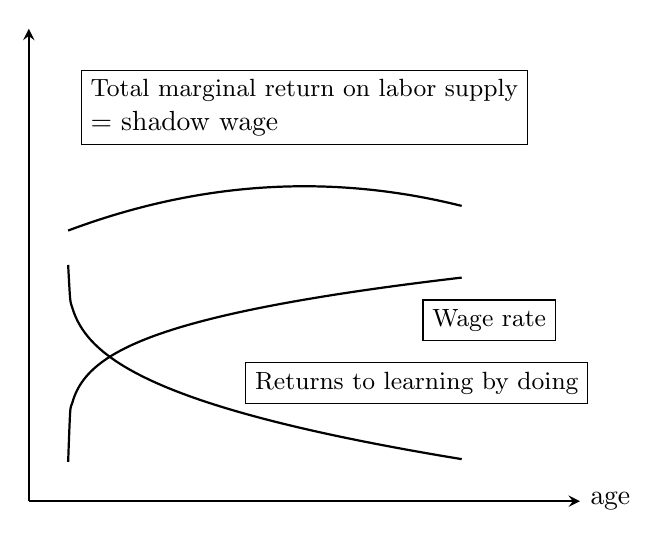
\begin{tikzpicture}
\draw[-stealth, black, thick] (0,0) -- (7,0) node[right] { age};
\draw[-stealth, black, thick] (0,0) -- (0,6);
\draw[thick, smooth, samples=200, xshift=.5cm, yshift=.5cm, domain=0:5] plot ({ \x, {(6*\x)^(1/4)}});
\node[right] at (5,2.3) [rectangle,draw] {\small Wage rate};
\draw[thick, smooth, samples=200, xshift=.5cm, yshift=3cm, domain=0:5] plot ({ \x, {-(3*\x)^(1/3)}});
\node[right] at (2.75,1.5) [rectangle,draw] {\small Returns to learning by doing};
% \draw[thick, smooth, samples=200, xshift=.5cm, yshift=2.5cm, domain=0.05:2.05] plot ({ \x, {\x^(1/2)-\x^(1/3)}});
\draw[thick, smooth, samples=200, xshift=-.5cm, yshift=2cm, domain=1:6] plot ({ \x, {2-(\x/4 - 1)^2}});
\node[align=left] at (3.5,5) [rectangle,draw] {\small Total marginal return on labor supply \\ = shadow wage};
\end{tikzpicture}
}
\caption{OPTIMAL LIFE CYCLE LABOR SUPPLY}
\label{fig:OptimalSupply}
\end{figure}
\end{frame}

\begin{frame}
  \frametitle{Table of Contents}
  \tableofcontents
\end{frame}
    
    \section{Model}
    \begin{frame}
      \frametitle{Agent's problem}
      Agents maximize their discounted expected life-cycle utility through the working horizon $T$:
      \begin{equation}
        \label{eq:LCU}
        % Eq. 1 from paper, discounted expected life cycle utility
E_t \sum_{\tau=t}^T \beta^{\tau} [u(C_{\tau} , \tau) - v(h_{\tau} \epsilon_{2,\tau})]
      \end{equation}
      subject to their intertemporal budget constraint:
            \begin{equation}
        \label{eq:IBC}
        % Eq. 2 from paper the IBC
A_{t+1} = (1 + r)A_t + W_{t,s}h_t - C_t
      \end{equation}
      Equations \eqref{eq:LCU} and equations \eqref{eq:IBC} characterize the problem we want to examine.
    \end{frame}

    \begin{frame}
      \frametitle{The human capital production function}
      \hypertarget{HCprodfunc}{}
      \begin{figure}[tbp]
        \centerline{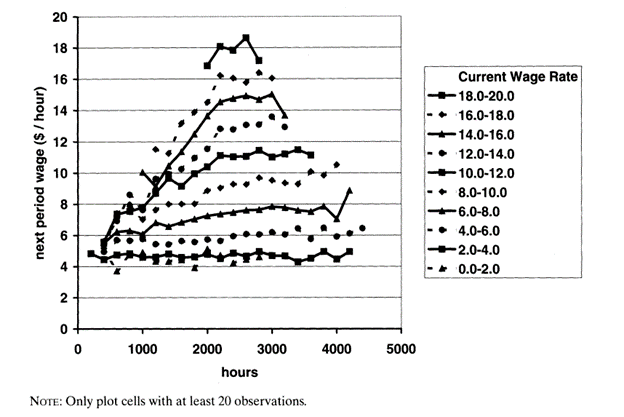
\includegraphics[width=4in]{\FigDir/Figure2}}
        \caption{HUMAN CAPITAL PRODUCTION FUNCTION} 
        \label{fig:HCprodfunc}
      \end{figure}
    \end{frame}

      \section{Solution}
      \begin{frame}
        \frametitle{Problem before shocks}
        Next period human capital before shocks are realized is:
        $$   \tilde{K}_{t+1} = g(h_t, K_t,t) $$
        So we can rewrite the value function as:
        \begin{equation*}
          \begin{split}
            V_{t,s}(A_t,\tilde{K}_t,\epsilon_{1,t},\epsilon_{2,t})=\text{max}_{C_t,h_t} & (u(C_t,t)-v(h_t, \epsilon_{2,t}) \\ & + \beta E_t V_{t+1,s+1} (A_{t+1},\tilde{K}_{t+1},\epsilon_{1,t+1},\epsilon_{2,t+1}))
          \end{split}
        \end{equation*}
      \end{frame}
      
    \begin{frame}
      \frametitle{Emax function}
      Defining the emax function as:
      \begin{equation}
        \label{eq:emax}
        % The e-max function is:
V^E_{t+1,s+1}(A_{t+1},\tilde{K}_{t+1}) = E_t V_{t+1,s+1}(A_{t+1},\tilde{K}_{t+1},\epsilon_{1,t+1},\epsilon_{2,t+1}) 
      \end{equation}
      We can write the agent's problem before shocks are realized as:
      \begin{align*}
& V_{t,s}(A_t, \tilde{K}_t,\epsilon_{1,t},\epsilon_{2,t}) = \\ & \text{max}_{C_t, h_t} [u(C_t,t) - v(h_t, \epsilon_{2,t}) + \beta V^E_{t+1,s+1} (A_{t+1},\tilde{K}_{t+1})]
        \end{align*}
  \end{frame}
  
  \section{Data}

   \begin{frame}
    \frametitle{NLSY79}
    \begin{enumerate}
    \item Our data comes from the NLSY79
    \item Advantage over the PSID, used by \cite{MaCurdy1981-iy} and others, is that we can directly use asset data
    \item Focus on white males who are at least 20 years old and have some schooling
    \end{enumerate}
  \end{frame}

  \begin{frame}
    \frametitle{Mean wage profiles}
    \centering
    \resizebox{!}{3.5cm}{%
      \begin{tabular}{l l l l}
        \hline%
        Age &  Hourly Wage &  Hours &  Total Wealth \\ \hline \\
       20 & 5.785 (2763) & 1531.7 (2837) & 6334.8 (207) \\ 
        21 & 5.998 (3220) & 1578.6 (3348) & 6178.5 (568) \\ 
        22 & 6.697 (3396) & 1725.7 (3536) & 8933 (956) \\ 
        23 & 7.12 (3420) & 1866.7 (3557) & 9163 (1361) \\ 
        24 & 7.342 (3308) & 1989.4 (3480) & 2889.9 (1751) \\ 
        25 & 7.99 (3187) & 2042 (3360) & -9276.6 (1885) \\ 
        26 & 9.294 (2987) & 2101.6 (3160) & 1205.6 (2189) \\ 
        27 & 9.098 (2871) & 2134.7 (3048) & 4651.3 (2504) \\ 
        28 & 10.1 (2785) & 2182.1 (2976) & -29888 (2538) \\
        29 & 9.426 (2499) & 2200.7 (2670) & -37101 (2235) \\ 
        30 & 12.36 (2028) & 2224.3 (2188) & -25726 (1903) \\ 
        31 & 15.24 (1649) & 2243.9 (1785) & -12168 (1614) \\ 
        32 & 13.6 (1206) & 2238.1 (1307) & 19201 (1313) \\ 
        33 & 22.98 (851) & 2253.1 (922) & 27379 (1098) \\ 
        34 & 11.39 (554) & 2246.7 (608) & 55264 (649) \\
        35 & 11.57 (291) & 2294.2 (325) & 84001 (299) \\
        36 & 10.01 (65) & 2283.5 (71) & 58172 (67) \\ 
        \\ \hline
        \multicolumn{4}{l}{NOTE: Sample sizes are in parentheses} 
      \end{tabular}
    }
  \end{frame}

  \section{Summary and Conclusion}

        \begin{frame}
    \frametitle{Intertemporal elasticities}
      \begin{itemize}
      \item Estimate the interemporal elasticity of labor supply of 3.82, much closer to that from the macro literature (eg \cite{Eichenbaum1988-kg})
      \item  Estimate an i.e.s.-c of -1.354
      \item This contrasts with the common estimate of -1/3 (see \cite{Hubbard1994-qp})
      \item Ignoring human capital biases IEL downwards and explains the dissonance between micro- and macro-estimates
    \end{itemize}
  \end{frame}

      \begin{frame}
      \frametitle{Model fit}
      \begin{figure}[tbp]
        \centerline{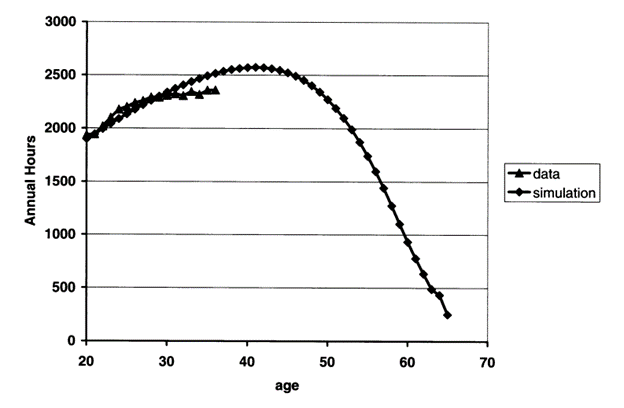
\includegraphics[width=4in]{\FigDir/Figure4}}
  \caption{AGE-HOURS PROFILES}
  \label{fig:AgeHoursProfiles}
      \end{figure}
    \end{frame}

          \begin{frame}
      \frametitle{Model fit}
      \begin{figure}[tbp]
        \centerline{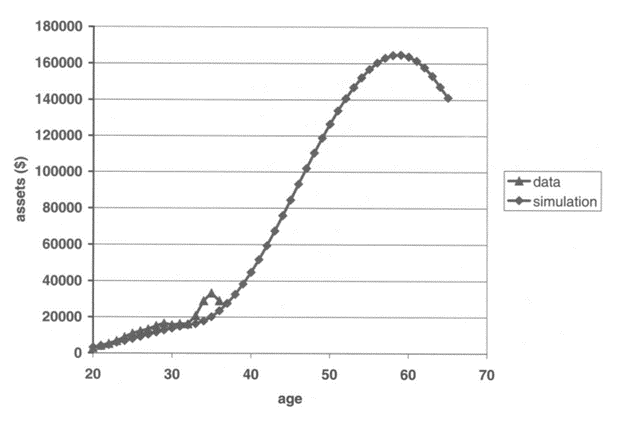
\includegraphics[width=4in]{\FigDir/Figure5}}
  \caption{AGE-ASSET PROFILES}
  \label{fig:AgeAssetProfiles}
      \end{figure}
          \end{frame}

          \begin{frame}[t, allowframebreaks]
            \frametitle{References}
            \bibliographystyle{amsalpha}
            \bibliography{ImaiKeane}
            \end{frame}
          
% \nobibliography{./ImaiKeane.bib}
  
\end{document}
